%Problem Set 1 LaTeX report for TDT4200
\documentclass[fontsize=11pt, paper=a4, titlepage]{article}
\usepackage{float} %For forcing position of figures
\usepackage{listings}	%For code in document
\usepackage[usenames,dvipsnames]{color}		%For the SkyBlue background color for lstlistings
\usepackage{mathtools}
\DeclarePairedDelimiter{\ceil}{\lceil}{\rceil}
\usepackage{amsfonts,amsmath,amssymb,amsthm}	%For \mathbb
% \usepackage{caption}	%Dunno yet
\usepackage{todonotes}	%For \todo
\usepackage{tabularx}	%for tablecontents wrapping inside cell, instead of cell breaking page width.
\usepackage{verbatim}
\usepackage{enumerate}	%For getting different types of lists like a) II) and so forth.
\usepackage[margin=2cm]{geometry}
\usepackage[utf8, utf8x]{inputenc}	%For norwegian letters and UTF8 encoding support
\usepackage{lastpage}	%For the command \pageref{lastpage}
\usepackage{fancyhdr}
\rfoot{\thepage\ / \pageref{LastPage}}

\usepackage{tikz}
\usepackage{colortbl}
\usetikzlibrary{calc}
\newcolumntype{W}{!{\smash{\vrule
\@width 4\arrayrulewidth
\@height\dimexpr\ht\@arstrutbox+2pt\relax
\@depth\dimexpr\dp\@arstrutbox+2pt\relax}}}
\makeatother
\definecolor{gray}{rgb}{.7,.7,.7}

\newcommand*\Laplace{\mathop{}\!\mathbin\bigtriangleup}

%\setlength{\parindent}{10ex}

\lstset{ %
language=C,							% choose the language of the code
basicstyle=\ttfamily,			% the size of the fonts that are used for the code
numbers=left,						% where to put the line-numbers
numberstyle=\footnotesize,			% the size of the fonts that are used for the line-numbers
stepnumber=1,						% the step between two line-numbers. If it is 1 each line will be numbered
numbersep=5pt,						% how far the line-numbers are from the code
backgroundcolor=\color{SkyBlue},	% choose the background color. You must add \usepackage{color}
showspaces=false,					% show spaces adding particular underscores
showstringspaces=false,				% underline spaces within strings
showtabs=false,						% show tabs within strings adding particular underscores
frame=single,						% adds a frame around the code
tabsize=4,							% sets default tabsize to 4 spaces
captionpos=b,						% sets the caption-position to bottom
breaklines=true,					% sets automatic line breaking
breakatwhitespace=false,			% sets if automatic breaks should only happen at whitespace
escapeinside={\%*}{*)}				% if you want to add a comment within your code
}

\lstset{literate=
	{á}{{\'a}}1 {é}{{\'e}}1 {í}{{\'i}}1 {ó}{{\'o}}1 {ú}{{\'u}}1
	{Á}{{\'A}}1 {É}{{\'E}}1 {Í}{{\'I}}1 {Ó}{{\'O}}1 {Ú}{{\'U}}1
	{à}{{\`a}}1 {è}{{\'e}}1 {ì}{{\`i}}1 {ò}{{\`o}}1 {ù}{{\`u}}1
	{À}{{\`A}}1 {È}{{\'E}}1 {Ì}{{\`I}}1 {Ò}{{\`O}}1 {Ù}{{\`U}}1
	{ä}{{\"a}}1 {ë}{{\"e}}1 {ï}{{\"i}}1 {ö}{{\"o}}1 {ü}{{\"u}}1
	{Ä}{{\"A}}1 {Ë}{{\"E}}1 {Ï}{{\"I}}1 {Ö}{{\"O}}1 {Ü}{{\"U}}1
	{â}{{\^a}}1 {ê}{{\^e}}1 {î}{{\^i}}1 {ô}{{\^o}}1 {û}{{\^u}}1
	{Â}{{\^A}}1 {Ê}{{\^E}}1 {Î}{{\^I}}1 {Ô}{{\^O}}1 {Û}{{\^U}}1
	{œ}{{\oe}}1 {Œ}{{\OE}}1 {æ}{{\ae}}1 {Æ}{{\AE}}1 {ß}{{\ss}}1
	{ç}{{\c c}}1 {Ç}{{\c C}}1 {ø}{{\o}}1 {å}{{\r a}}1 {Å}{{\r A}}1
	{€}{{\EUR}}1 {£}{{\pounds}}1
}
 %config.tex file in same directory for all reports

\begin{document}

\begin{center}

{\huge Problem Set 3, Theory}\\[0.5cm]

\textsc{\LARGE TDT4200 -}\\[0.5cm]
\textsc{\large Parallel Computations}\\[1.0cm]

\begin{table}[h]
    \centering
    \begin{tabular}{c}
        \textsc{Christian Chavez}
    \end{tabular}
\end{table}

\end{center}
\vfill
\hfill \large{\today}
\clearpage

\section{Problem 1, MPI derived types}

\begin{enumerate}[a)]

    \item MPI communication mechanisms at its basic level can be used to send or
receive a sequence of identical elements that are contiguous in memory. However,
you would often want to send datat that is either not homogenous, or not
contiguous (like the subdomains of the previous coding assignment) in memory.

Derived datatypes in MPI are used to send such types of data. This alleviates
the option of having the overhead of sending or receiving a message transmitting
many elements, or having to ``pack'' the data in a temporary contiguous buffer
on the sending process, and then ``unpacking'' the data again from an an
identical contiguous buffer in the receiving process.

    \item See below picture for answer to this subproblem.
        \begin{figure}[H]
            \centering
            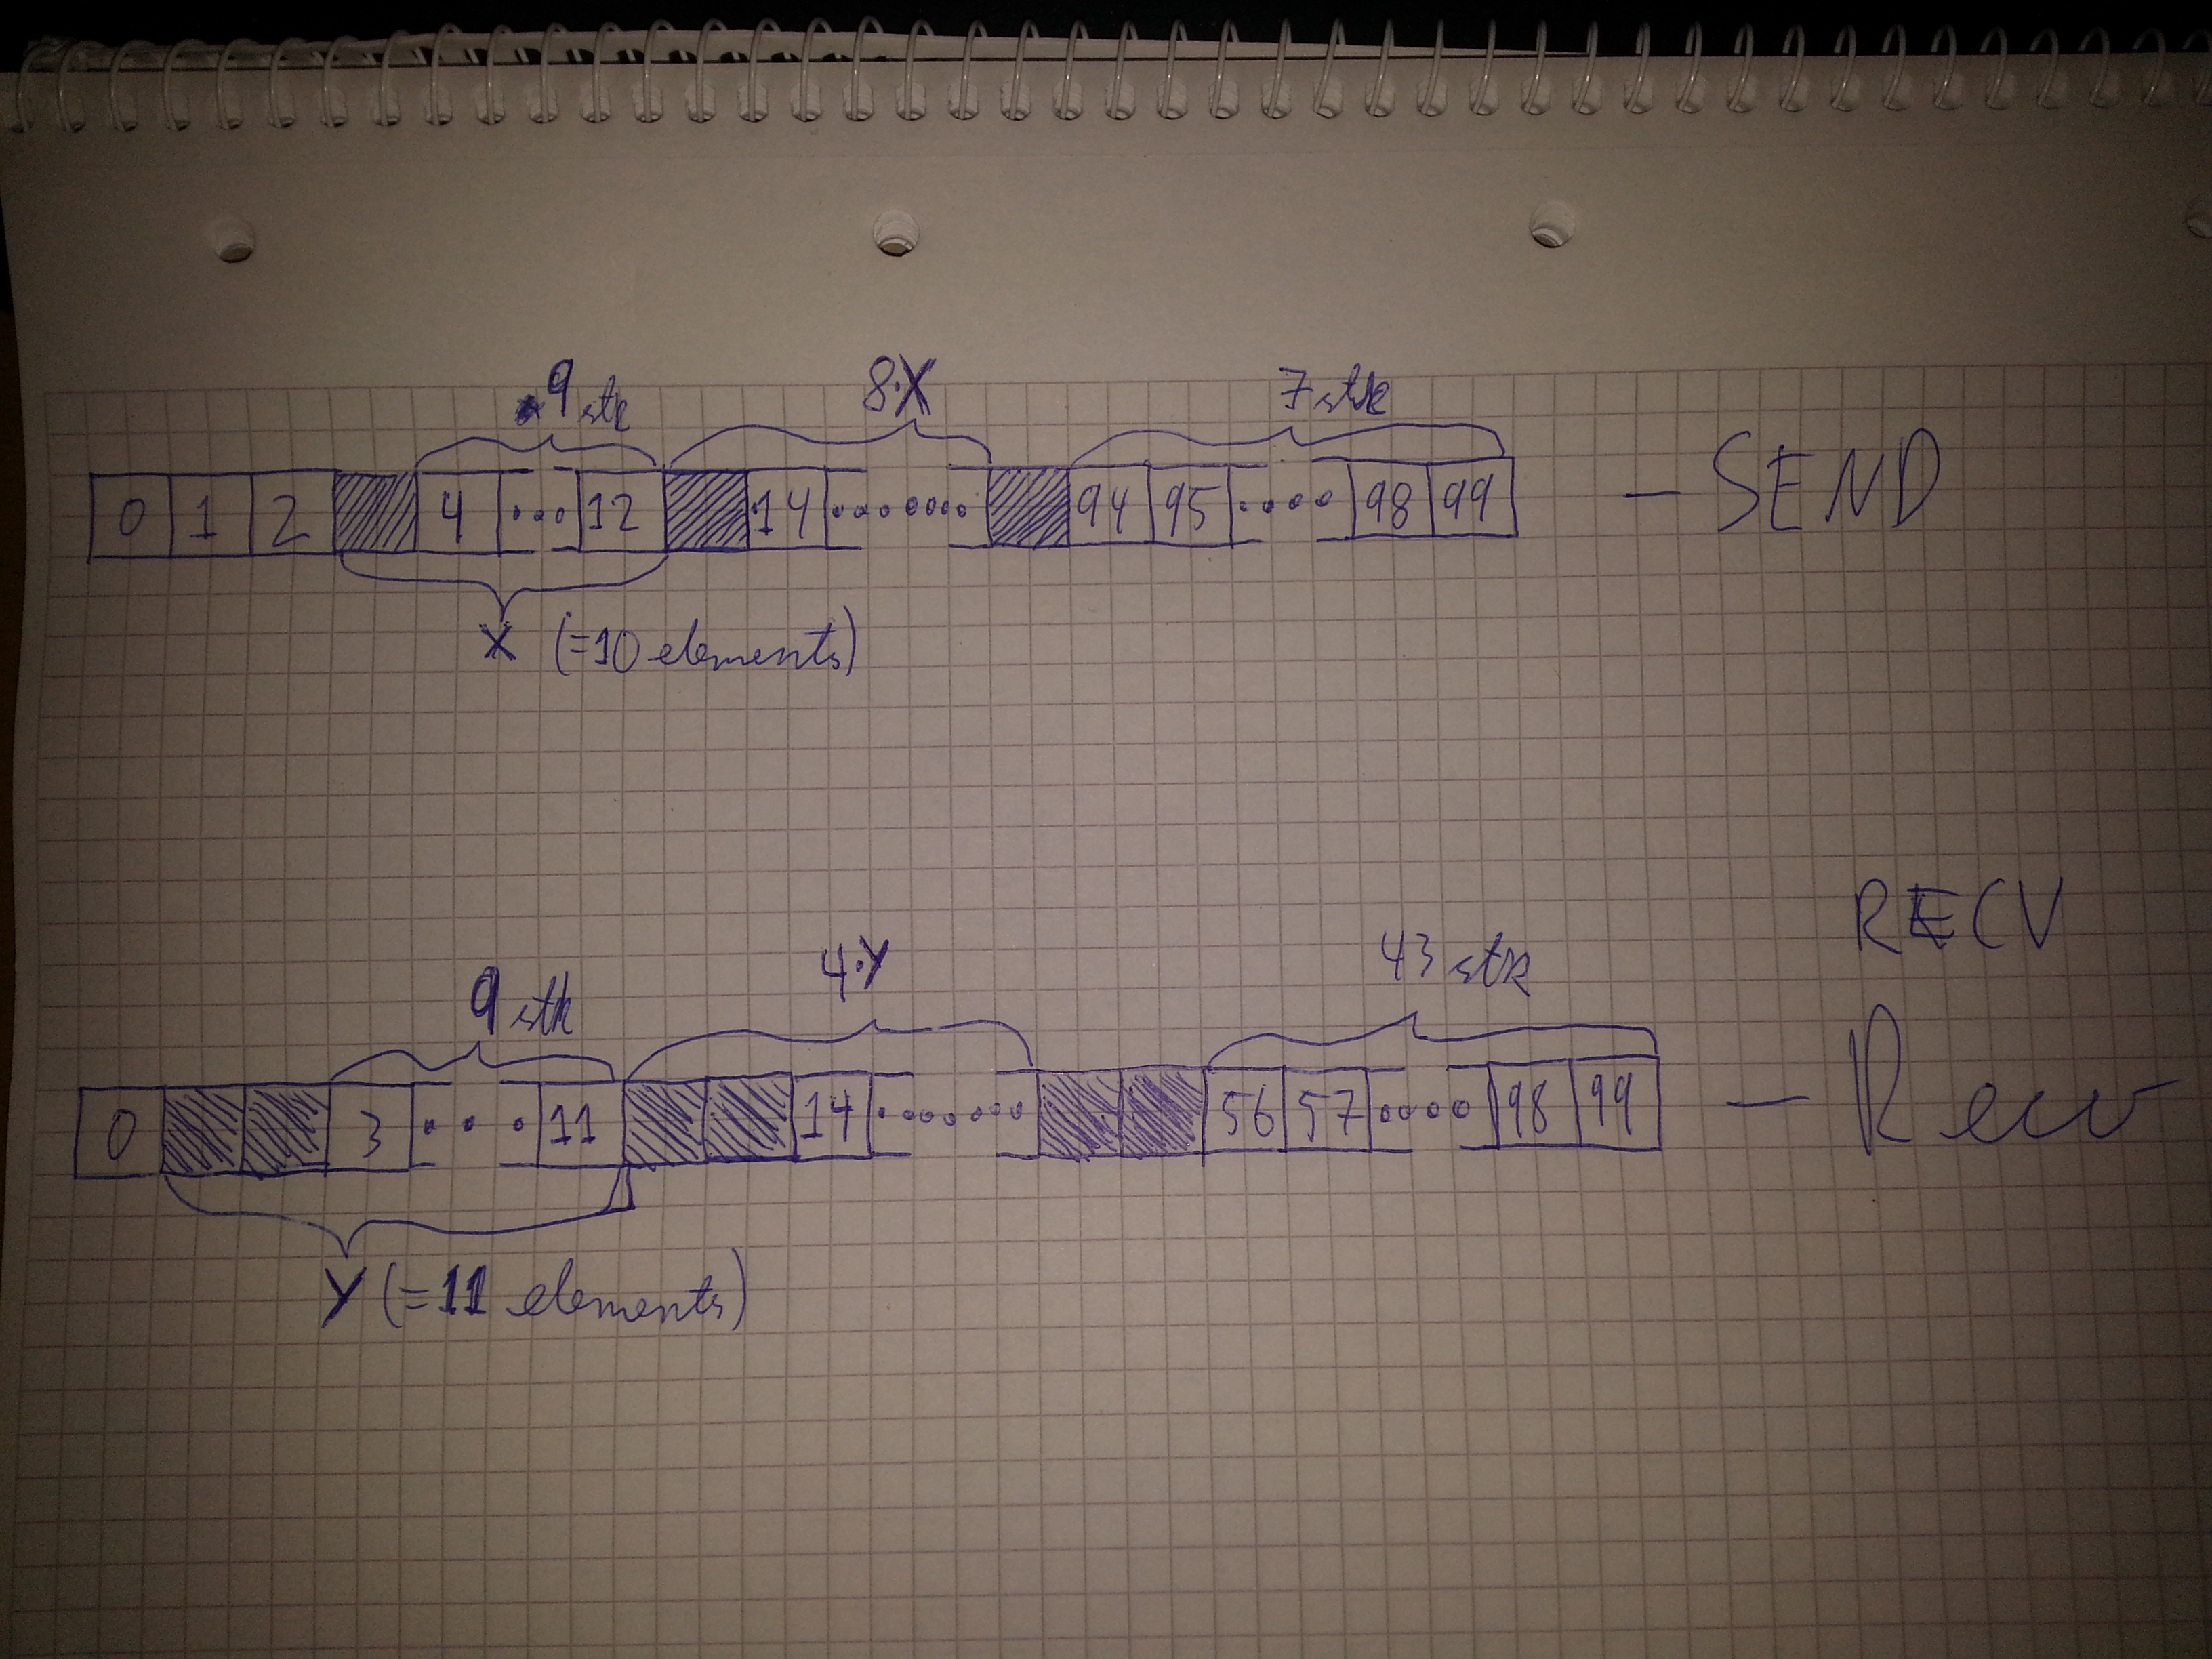
\includegraphics[width=1.0\linewidth]{1b.jpg}
            \caption{Data placement in arrays}
            \label{fig:1b}
        \end{figure}
    NB: The transferred elements (filled boxes) are received in the same order
as they are sent. The first one in the send array is also the first one in
the receive array, and so on.


\end{enumerate}

\section{Problem 2, Memory and Caching}

\begin{enumerate}[a)]

    \item The three types of cache misses are \textit{Compulsory},
\textit{Capacity}, and \textit{Conflict}.
    \begin{enumerate}[I)]

        \item \textbf{Compulsory} cache misses happens when the data is not
already stored in the cache, and needs to be retrieved from a lower level memory
of the memory hierarchy (like RAM).

        \item \textbf{Capacity} cache misses happen when the cache is full, and
the data is not in cache. Meaning that due to the finite size of cache,
something else needs to be evicted to make space for the new data.

        \item \textbf{Conflict} cache misses happen when the data requested at
some earlier point was present in cache, but was then later (but before the new
request) evicted. So in other words, a cache miss that could have been avoided.

    \end{enumerate}

    \item Temporal locality refers to references to the same part of memory in
close temporal proximity (near future). That instead of referring to variable
\textit{X} 7 times equidistantly spread throughout the programflow, you refer to
it 7 times in a row. (Simplified example.)

The concept that likelihood of referencing a resource is higher if a resource
near it was just referenced.

Spatial locality is the same thing, except here it's about which memory space
you're addressing, not when. So if one part of memory is referenced, spatial
locality is when memory near this reference has a higher chance of also being
accessed.

    \item Assumption \textbf{1}: That the cache is not big enough to fit all
three arrays in cache, since three identical int arrays of size $100 000$ each,
with an int being $16$ bits long, would imply a cache size of $\approx 9.16$
Mbit cache. Hence, spatial locality will never be possible for all full three
arrays at the same time.

Assumption \textbf{2}: The cache blocks are $64$ bytes in size, meaning that
when a subset of the above arrays are loaded in, at most $16$ values of that
subsection of the array is loaded into the cache.

    \begin{enumerate}[I)]

        \item Since this for-loop jumps to every thousandth indice, there is no
spatial locality at play, if assumption \textbf{2} holds. $(16 \ll 1000)$.
Neither is there temporal locality, since the instructions the for-loop repeats
change the data locations they're repeated on for every iteration.

        \item This pattern exhibits spatial locality since it's accessing each
indice in turn, not jumping over indices too big for the suggested size of a
cache block. There is, however no temporal locality, since the same memory
address is only referenced once.

        \item This pattern exhibits temporal locality, but not spatial locality.
Temporal because of the outer for-loop, which makes the inner for-loop re-
reference the memory addresses a $100$ times each. But since each reference is
at a minimum a $1000$ elements away from each other, and if assumption
\textbf{2} holds, then there is absolutely no spatial locality.

    \end{enumerate}
\end{enumerate}

\section{Problem 4, Branching}
\begin{enumerate}[a)]

    \item \textit{Branch prediction} is when a prediction is made regarding
which  option an if-clause will choose, so that the data of the (hopefully correctly chosen if-clause) can be already loaded into cache when it's needed.

If the prediction made is correct, then there can be performance improvement due
to the data already being in cache when referenced the first time, due to the
data being loaded at the preceding if-clause.

    \item Total time for code execution $T_{tot}$:
    \begin{align*}
        T_{tot} &= n((p+f)r + (1-r)(p+s))
    \end{align*}

    \begin{enumerate}[I)]

        \item By setting the time cost of running all iterations through the
slow function $(p+s)n$ to be less than the total run-cost $T_{tot}$, we can find
the value $r$ has to be to make this a beneficial trade. But since the branch
predictor always assumes the if-clause to return false, we need to add the
branch prediction cost $b$ for the fast alternative.

        \begin{align*}
            sn &< n((p+b+f)r + (1-r)(p+s)) \\
            s &< (p+b+f)r + (p+s) - r(p+s) \\
            -p &< (p+b+f)r - r(p+s) \\
            p &> r((p+s) - (p+b+f)) \\
            p &> r(s-b-f) \\
            \frac{p}{(s-b-f)} &< r
        \end{align*}

$r$ has to be bigger than $\frac{p}{s-b-f}$ for the code to be faster by
running all the iterations through the slow function, instead of keeping the if-
clause. This relies on $s \ge p+b+f$, otherwise $r$ will not be positive with
a value between $0$ and $1$.

    \item If the branch predictor always mispredicts, $T_{tot}$ then becomes
$T_{tot} = n(r(f+b+p) + (1-r)(s+b+p))$. When setting the new $T_{tot}$ to take
longer time than just using the slow function, $r$ has to be:

        \begin{align*}
            sn &< n(r(f+b+p) + (1-r)(s+b+p)) \\
            s &< r(f+b+p) + (s+b+p) -r(s+b+p) \\
            s - (s+b+p) &< r(f-s) \\
            (b+p) &< r(s-f) \\
            \frac{b+p}{s-f} &< r
        \end{align*}

    \end{enumerate}
\end{enumerate}

\section{Problem 5, Optimization}
\begin{enumerate}[a)]

    \item If the table is sufficiently big so that a look-up in the table takes
sufficient time (e.g. does not fit in cache), the code might get slowed down by this ``optimization''.

However, if the table isn't too big (fits in cache), and say is possible to
access like a hash table in $O(1)$ time, then that will be faster than a
function that which is slow to compute the return value.

    \item Assumption \textbf{1}: \textit{f()} returns ints, of $32$ bits length.

Assumption \textbf{2}: Time it takes to index table is constant/inconsequential,
no matter the size.

Assumption \textbf{3}: Hit rate of cache in this problem,
given table size, is simply $\frac{cache\thickspace size}{table\thickspace size}$.

Given assumptions \textbf{1}, \textbf{2}, and \textbf{3}, this question asks how
big the cache must be, so that the cache misses are few enough, such that it
will be faster to replace \textit{f()} with a table.

Since \textit{f()} in the example only receives values between $0$ and
$(127\times 128) + 1024 = 17\thickspace 280$, the table size does not have to
fit more ints than this. Total table size (denoted as $S$) then has to be equal
or greater than $17\thickspace 280*32 = 552\thickspace 960$ to fit all the
(potentially) different return values.

Cache size will be denoted as $X$. The time the code requires to execute with
\textit{f()} will be denoted as $T_f$, and the time the code requires to execute
with the table will be denoted as $T_t$.

    \begin{align*}
        T_{f()} = T_f &= 128\times 4\times 1024\times 5h
        = 2\thickspace 621\thickspace 440h \\
        T_{table} = T_t &= hS\times(\frac{X}{S} + (1-\frac{X}{S})10)\\
        T_t &= h(10S- 9X)
    \end{align*}

Hence, the equation becomes:

    \begin{align*}
        T_t &< T_f \\
        h(10S-9X) &< 2\thickspace 621\thickspace 440h \\
        10S - 9X &< 2\thickspace 621\thickspace 440 \\
        10\times 552\thickspace 960 - 9X &< 2\thickspace 621\thickspace 440 \\
        9X &< 10\times 552\thickspace 960 - 2\thickspace 621\thickspace 440 \\
        9X &> 2\thickspace 908\thickspace 160 \\
        X &> \frac{2\thickspace 908\thickspace 160}{9}
    \end{align*}

With a value for $X$ in bits, we can then divide this by $64\times 8 = 512$ to
find out how many cache lines $c$ are necessary to have a sufficiently large
cache:

    \begin{align*}
        c &= \frac{\frac{2\thickspace 908\thickspace 160}{9}}{512} \\
        c &= \frac{5680}{9} \approx 631.10
    \end{align*}

The cache must be a minumum of $632$ cache lines big, where each cache line is
$64$ bytes long. This results in a minimum of $323\thickspace 584$ bits
necessary cache size for replacing \textit{f()} with a table to be an
improvement.

\end{enumerate}

\vfill
\hfill \large{\today}
\end{document}
